

% \usepackage[utf8]{inputenc} % allow utf-8 input
% %\usepackage[T1]{fontenc}    % use 8-bit T1 fonts (forbidden by AAAI)
% %\usepackage{hyperref}       % hyperlinks
% \usepackage{booktabs}       % professional-quality tables
% \usepackage{amsfonts}       % blackboard math symbols
% \usepackage{nicefrac}       % compact symbols for 1/2, etc.
% \usepackage{microtype}      % microtypography
% \usepackage{mathtools}
% \usepackage{afterpage}
% \usepackage{parselines}
% \usepackage{verbatim}
% \usepackage[ruled]{algorithm2e}
% \usepackage{amsmath}


\documentclass{article}


\usepackage{arxiv}

\usepackage[utf8]{inputenc} % allow utf-8 input
\usepackage[T1]{fontenc}    % use 8-bit T1 fonts
% \usepackage{hyperref}       % hyperlinks
\usepackage{url}            % simple URL typesetting
\usepackage{booktabs}       % professional-quality tables
\usepackage{amsfonts}       % blackboard math symbols
\usepackage{nicefrac}       % compact symbols for 1/2, etc.
\usepackage{microtype}      % microtypography
\usepackage{lipsum}
\usepackage{graphicx}
\usepackage{amsmath}


\title{Clustered Hierarchical Anomaly and Outlier Detection Algorithms}


\author{
    Najib Ishaq \\
    Department of Computer Science and Statistics\\
    University of Rhode Island\\
    Kingston, RI\\
    \texttt{najib\_ishaq@uri.edu} \\
    \And
    Thomas J. Howard III \\
    Department of Computer Science and Statistics\\
    University of Rhode Island\\
    Kingston, RI\\
    \texttt{thoward27@uri.edu} \\
    \AND
    Noah M. Daniels \\
    Department of Computer Science and Statistics\\
    University of Rhode Island\\
    Kingston, RI\\
    \texttt{noah\_daniels@uri.edu} \\
}

\begin{document}
    \maketitle

    \begin{abstract}
        Anomaly and outlier detection in datasets is a long-standing problem in machine learning.
        In some cases, anomaly detection is easy, such as when data are drawn from well-characterized distributions such as the Gaussian.
        However, when data occupy high-dimensional spaces, anomaly detection becomes more difficult.
        We present CLAM (Clustered Learning of Approximate Manifolds), a fast hierarchical clustering technique that learns a manifold in a Banach space defined by a distance metric.
        CLAM induces a graph from the cluster tree, based on overlapping clusters drawn from a cluster-tree determined by several geometric and topological features.
        Upon several such graphs we implement CHAODA (Clustered Hierarchical Anomaly and Outlier Detection Algorithms), exploring various properties of the graphs and their constituent clusters in order to compute scores of anomalousness.
        On 24 publicly available datasets, we compare the performance of CHAODA (by measure of the AUC of a ROC curve) to a variety of state-of-the-art unsupervised anomaly-detection algorithms.
        Six of the datasets are used for training.
        Of the remaining 18, CHAODA outperforms other approaches on 14 datasets.
    \end{abstract}

    \section{Introduction}
\label{sec:introduction}

TODO

%Detecting anomalies and outliers from data is a well-studied problem in machine learning.
%When data occupy easily-described distributions, such as the Gaussian, the task is relatively easy: one need only identify when a datum is sufficiently far from the mean.
%However, in ``big data'' scenarios, where data can occupy high-dimensional spaces, anomalous behavior becomes harder to quantify.
%If the data happen to be uniformly distributed, one can conceive of simple mechanisms, such as a one-class SVM, that would be effective in any number of dimensions.
%However, real-world data are rarely distributed uniformly.
%Instead, data often obey the ``manifold hypothesis''~\cite{fefferman2016testing}, occupying a low-dimensional manifold in a high-dimensional embedding space.
%This low-dimensional manifold may weave itself through the high-dimensional space much like a crumpled sheet of paper does in 3-dimensional space.
%Detecting anomalies in such a landscape is not easy;
%in particular, correctly identifying an anomalous datum that sits within the gaps of a lower-dimensional manifold presents a challenge.
%
%Anomalies (data that do not belong to a distribution) and outliers (data which represent extrema of a distribution) can arise from many sources:
%errors in measurement or collection of data;
%novel, previously-unseen instances of data;
%normal behavior evolving into abnormal behavior;
%and adversarial attacks as inputs to machine-learning algorithms~\cite{elsayed2018adversarial}.
%Modern algorithms designed to detect anomalous behavior fail for a variety of reasons, in particular when anomalies live close to, but not on, a complex manifold in high-dimensional space.
%Our approach is designed to learn these complex manifolds.
%Here we briefly survey contemporary approaches to anomaly detection in order to provide the context needed to understand how our approach differs.

    \section{Methods}
\label{sec:methods}

\subsection{CLAM}
\label{subsec:methods:clam}

We present a Manifold-Mapping algorithm called CLAM (Clustered Learning of Approximate Manifolds).
This is an extension of earlier work presented in~\cite{ishaq2019clustered}.

To start, we need a dataset and a distance function on the points in that dataset.
A dataset is a collection of $n$-points in a $D$-dimensional embedding space.
\begin{gather*}
    \textbf{X} = \{x_1 \dots x_n\}, x_i \in \mathbb{R}^D
\end{gather*}
A Distance Function takes two points in the dataset and deterministically produces a non-negative real number.
\begin{gather*}
    f : (\mathbb{R}^D, \mathbb{R}^D) \mapsto \mathbb{R}^+
\end{gather*}
We require any distance function to have the following properties:
\begin{align*}
    \forall x \in X,    & \ f(x, x) = 0       \\
    \forall x, y \in X, & \ f(x, y) = f(y, x)
\end{align*}
The distance function may or may not obey the triangle-inequality.

\subsubsection{Clustering:}\label{subsubsec:methods:clam:clustering}
% describe creation of Cluster Tree
We start by building a divisive-hierarchical clustering of the data based on a random sampling of $\sqrt(k)$ datapoints, for $k$ points at a given level of the tree, which achieves clustering in expected $\mathcal{O}(n \lg n)$ time.
This gives us a tree of clusters, with the root containing every point in the dataset, and each leaf containing a single point from the dataset.
The procedure is detailed in~\cite{ishaq2019clustered}.

Several properties of clusters are interesting and important to consider, including \textit{cardinality}, the number of points in a cluster; \textit{center}, the geometric median of points contained in a cluster; \textit{radius}, the distance to the farthest point from a center; and \textit{local fractal dimension}, as described in~\cite{ishaq2019clustered}.
We can also consider individual \textit{parent-child ratios} of cardinality, radius, and local fractal dimension, as well as \textit{exponential moving averages} of the parent-child ratios along a branch of the tree.
In particular, we use the parent-child ratios and the exponential moving averages of those ratios to help generalize our anomaly detection method from a small set of datasets to a large, distinct set of datasets.
/
\subsubsection{Graphs:}
% TODO: describe Graph and graph invariant.
Clusters that are near each other in the embedding space sometimes have overlapping volumes, i.e.\ the distance between their centers is less than or equal to the sum of their radii.
We define a graph $G=(V,E)$ with the selected clusters in one-to-one correspondence to vertices, and with an edge between two vertices if and only if their corresponding clusters overlap.
For our purposes, a graph also exhibits a particular invariant:
\begin{itemize}
    \item The clusters corresponding to vertices in the graph collectively contain every point in the dataset.
    \item Each point in the dataset is in exactly one cluster corresponding to exactly one vertex in the graph.
\end{itemize}
A corollary to this invariant is that the graph will never contain two vertices such that one vertex corresponds to a parent or child cluster of another vertex.
% Go over layer-graphs and optimal-graphs.
A Graph can be built from clusters at a fixed depth in the cluster-tree (a layer-graph), or from clusters from multiple different depths in the tree (an optimal-graph).
In this work we consider the cardinality of a graph to be \textit{vertex cardinality}, i.e.\ the number of vertices (clusters) in the graph.

\subsubsection{The Manifold:}
% describe Manifold as containing the tree and all the graphs.
According to the Manifold Hypothesis~\cite{fefferman2016testing},
datasets that come from constrained generating processes and are embedded in a high-dimensional space actually only occupy a low-dimensional manifold in that embedding space.

The graphs discussed so far map this low dimensional manifold in the original embedding space.
Different graphs do this at different levels of local and/or global resolution.
Our aim is to properly build such a graph, where different levels of resolution may be necessary for different regions of the manifold.
We can then apply several anomaly detection algorithms to these graphs.
These algorithms will often also incorporate information from the tree, such as parent-child cardinality ratios.

We describe some algorithms in Section~\ref{subsec:methods:individual-algorithms}.
While these algorithms are themselves fairly simple, the real challenge is in selecting the right clusters for the graphs for the algorithms operate on.
We will demonstrate CLAM to be such a powerful technique in Manifold-Mapping that even these simple algorithms, more often than not, outperform state-of-the-art anomaly detection algorithms.

\subsection{Induced Graphs:}
\label{subsec:methods:induced-graphs}
The heart of the problem with our methods of anomaly detection is building the right graph to represent the underlying manifold.
One could try using every possible combination of clusters to form a graph but this quickly leads to combinatorial explosion.
Instead, we must intelligently select those clusters that, when used to build the graph, perform best for anomaly detection.

Area Under the Curve (AUC) of the Receiver Operating Characteristic (ROC) is often used to measure the performance of anomaly detectors;
we wish to choose clusters that are expected to maximize this measure.
We can accomplish this by learning a function that takes a cluster and predicts its contribution to AUC if that cluster were selected for the graph.
Any function of the following form will suffice.
\begin{gather*}
    f: Cluster \mapsto \mathbb{R}^+
\end{gather*}

We chose a simple linear regression to fill this role.
Such a model needs some data to train with.
To generate this data, we took a random sample of some of the datasets described in Section~\ref{subsec:methods:datasets}, choosing six datasets at random which had at between 1000 and 100,000 samples.
We generate CLAM Manifolds for these training datasets, use the linear regression model to learn from these datasets, and apply the results to an entirely different collection of datasets. The process is as follows.

We generate the initial training data by considering layer-graphs.
For each such graph, we calculate the means of the cardinality ratio, radius ratio, and local fractal dimension ratio;
along with the exponential moving averages of these ratios, described in Section~\ref{subsubsec:methods:clam:clustering}.
These ratios form the feature vector for one training sample.
For each method described in Section~\ref{subsec:methods:individual-algorithms}, we apply it to the graph and obtain an AUC ROC\@.
We then train the regression model to predict this AUC from the features extracted from the graph.
The result is a separate regression model for each algorithm of CHAODA.


% describe individual algorithms.
\subsection{Individual Algorithms}\label{subsec:methods:individual-algorithms}

Here we describe several simple methods for anomaly detection.
Each of these methods uses a graph of clusters from CLAM to calculate an anomalousness score for each point in the dataset.

For each algorithm:
\begin{itemize}
    \item $scores$ is a dictionary of clusters and their outlier scores,
    \item $V$ is the set of clusters in a graph,
    \item $E$ is the set of edges in a graph, And
    \item the cardinality of a cluster $c$ is denoted by $|c|$, represneting the number of points in a cluster.
\end{itemize}

\subsubsection{Relative Cluster Cardinality:}
We measure the anomalousness of a point by the cardinality of the cluster that point belongs to relative to the cardinalities of the other clusters in the graph.
Points in the same cluster are considered equally anomalous and points in clusters with relatively low cardinalities are considered more anomalous than points in clusters with relatively high cardinalities.

The algorithm is as follows:

\begin{itemize}
    \item for each cluster $c$ in graph $g$:
    \begin{itemize}
        \item $scores[c] \leftarrow -|c|$.
    \end{itemize}
\end{itemize}

The time complexity of this algorithm is $O(|V|)$.

\subsubsection{Relative Component Cardianlity}
We define components of a graph by the property that no two clusters from different components have an edge between them, and every pair of clusters in the same component has a path between them.
Consider the relative cardinalities of each component in much the same we we considered the relative cardinalities of clusters in the Relative Cluster Cardinality method.
Points in clusters in relatively small components are considered more anomalous than points in clusters in relatively large components, and points in clusters in the same component are considered equally anomalous.

The algorithm is as follows:

\begin{itemize}
    \item for each component $C$ in graph $g$:
    \begin{itemize}
        \item for each cluster $c$ in $C$:
        \begin{itemize}
            \item $scores[c] \leftarrow -|C|$.
        \end{itemize}
    \end{itemize}
\end{itemize}

This algorithm first finds the components of the graph, so its time complexity is $O(|E| + |V|)$.

\subsubsection{Graph Neighborhood Size:}
Given the graph with clusters and edges, consider the number of clusters reachable from a starting cluster within a given graph distance $k$.
We call this number the \textit{graph-neighborhood} of the starting cluster.
With $k$ relatively small compared to the diameter of the graph, we can consider the relative sizes of \textit{graph-neighborhood} of the clusters in the graph.
Points in clusters with small graph-neighborhoods are considered more anomalous than points in clusters with large graph-neighborhoods.

The algorithm is as follows:

\begin{itemize}
    \item let $f$ be a real number in the $(0, 1]$ range ($0.25$) works well.
    \item for each cluster $c$ in graph $g$:
    \begin{itemize}
        \item let $e_c$ be the eccentricity of $c$.
        \item let $s$ be $e_c * f$.
        \item perform a breadth-first traversal from $c$ with $s$ steps.
        \item let $size$ be the number of unique clusters visited by the breadth-first traversal.
        \item $scores[c] \leftarrow -size$.
    \end{itemize}
\end{itemize}

This algorithm is dominated by the computation of the eccentricity of each cluster.
Its time complexity is $O(|E| \cdot |V|)$.

\subsubsection{Child-Parent Cardinality Ratio:}
As described in CHESS~\cite{ishaq2019clustered}, a cluster is partitioned by using its two maximally distant points as poles.
The points are split among children by whichever pole they are closer to.
Consider the fraction of points in a cluster that are assigned to each child.
If a child cluster only contains a small fraction of the points that its parent did, then we consider the points in that child cluster to be anomalous.
These child-parent cardinality ratios are accumulated for each point down its branch in the tree, terminating when the child cluster is a node in the graph.
Points with a low value of these accumulated ratios are considered more anomalous than points with a high value of these accumulated ratios.

The algorithm is as follows:

\begin{itemize}
    \item for each cluster $c$ in graph $g$:
    \begin{itemize}
        \item let $p$ be the parent cluster of $c$.
        \item $scores[c] \leftarrow \frac{|p|}{|c|}$.
    \end{itemize}
\end{itemize}

The time complexity of this algorithm is $O(|V|)$.


\subsubsection{Random Walks:}
We perform long random-walks on each component of a graph, and we count the number of times each cluster was visited.
We consider the relative visitation counts among the clusters to be inversely related to their anomalousness.
The least visited clusters are anomalous, and the most visited clusters are not.

The algorithm is as follows:

\begin{itemize}
    \item let $visits$ be a dictionary of clusters and their visitation counts, initialized to $0$.
    \item let $s$ be a large number of steps for the random walk.
    \item for each cluster $c$ in graph $g$:
    \begin{itemize}
        \item perform a random walk from $c$ with $s$ steps and increment the value of the visited cluster in $visits$ with each step.
    \end{itemize}
    \item for each cluster $c$ in graph $g$:
    \begin{itemize}
        \item $scores[c] \leftarrow -visits[c]$.
    \end{itemize}
\end{itemize}

This algorithm is dominated by the computation of the transition matrix for the graph.
Its worst-case time complexity is $O(|V|^2)$, but is often better because the transition matrix is computed separately for each component in the graph.

\subsubsection{Stationary Probabilities:}
We compute the transition probability matrix of each component of a graph that contains at least two clusters.
We then compute successive powers of this matrix.
This process will eventually converge (add citation here), and we find this convergent matrix.
The sum of the values along a row is inversely related to the anomalousness of the respective cluster.

The algorithm is as follows:

\begin{itemize}
    \item for each component $C$ in graph $g$:
    \begin{itemize}
        \item let $M$ be the transition matrix for $C$.
        \item keep squaring $M$ until the matrix converges.
        \item let $S$ be this converged matrix.
        \item for each cluster $c$ in $C$:
        \begin{itemize}
            \item let $s$ be the respective row from $S$.
            \item $scores[c] \leftarrow -sum(s)$
        \end{itemize}
    \end{itemize}
\end{itemize}

This algorithm is dominated by the computation of the transition matrix for each component in the graph.
Its time worst-case time complexity is $O(|V|^2)$, but is often better in practice.


\subsection{Normalization}\label{subsec:methods:normalization}
The individual methods produce outlier scores for each cluster, rather than for each point.
We remedy this by having each point simply inherit the outlier score of the cluster it belongs to.
Since our graphs guarantee that each point is in exactly one cluster, and that every point from the dataset is accounted for, this inheritance assigns an outlier score to each point in a dataset.

However, the individual methods still produce outlier scores in a wide range of values.
The only common feature among these scores is that low scores correspond to inliers and high scores correspond to outliers.
Thesefore, scores from differnt methods or graphs cannot be directly compared to each other.
We need some method for normalizing these scores to the same range.
The standard range is $[0, 1]$, with high scores assigned to outliers.

We use gaussian normalization by default, though we include sigmoid normalization and min-max normalization as options in our implementation. (add possible citation for paper on normalizing such scores)

% TODO: Add equations and/or citations for normalization methods.

Once the scores are in a uniform range, we are ready for the ensemble.


\subsection{Ensemble}\label{subsec:methods:ensemble}
Given the set of regression models learned from the training datasets described in Section~\ref{subsec:methods:induced-graphs}, we can use it to build graphs for any other dataset, even if those datasets differ significantly in dimensionality and size; essentially, this is a form of transfer learning.
We use the cluster ratios and the associated regression constants to rank every cluster in a CLAM tree.
These rankings are normalized by the cardinality of each cluster.
The highest ranked clusters are then used to build a graph.
This graph is then used with the corresponding individual algorithm to calculate anomaly scores for all points in the dataset.
The scores from each individual algorithm are then combined into an ensemble.
We present the AUC scores from this ensemble in Section~\ref{sec:results}.

% TODO: Add a note on speed and the settings between CHAODA-fast and CHAODA


\subsection{Datasets}\label{subsec:methods:datasets}

We sourced 24 datasets, all from Outlier Detection Datasets (ODDS)~\cite{rayana2016odds}, for training CHAODA and testing its performance.
All of these datasets are adapted from the UCI Machine Learning Repository (UCIMLR)~\cite{UCIMLR}, and have been standardized, by ODDS, for anomaly and outlier detection benchmarks.

We provide a summary of the datasets in table~\ref{table:methods:benchmarks}.
For more details on each dataset, please refer to the supplementary materials.

\begin{table*}[!t]
\renewcommand{\arraystretch}{1.25}
\caption{Datasets used for Benchmarks}
\label{table:methods:benchmarks}
\centering
\begin{tabular}{|c|c|c|c|}
\hline
\textbf{Dataset} & \textbf{Cardinality} & \textbf{Dimensionality} & \textbf{\# Outliers} \\
\hline
annthyroid & 7,200 & 6 & 534 \\
\hline
arrhythmia & 452 & 274 & 66 \\
\hline
breastw & 683 & 9 & 239 \\
\hline
cardio & 1,831 & 21 & 176 \\
\hline
cover & 286,048 & 10 & 2,747 \\
\hline
glass & 214 & 9 & 9 \\
\hline
http & 567,479 & 4 & 2,211 \\
\hline
ionosphere & 351 & 33 & ?? \\
\hline
lympho & 148 & 18 & 6 \\
\hline
mammography & 11,183 & 6 & 260 \\
\hline
mnist & ?? & 100 & 700 \\
\hline
musk & 3,062 & 166 & ?? \\
\hline
optdigits & 5,216 & 64 & 150 \\
\hline
pendigits & 6,870 & ?? & 156 \\
\hline
pima & ?? & ?? & ?? \\
\hline
satellite & 6,435 & 36 & ?? \\
\hline
satimage-2 & 5,803 & 36 & 71 \\
\hline
shuttle & 59,097 & 9 & 3,511 \\
\hline
smtp & 95,156 & 3 & 30 \\
\hline
thyroid & 3,772 & 6 & 93 \\
\hline
vertebral & 240 & 6 & 30 \\
\hline
vowels & 1,456 & 12 & 50 \\
\hline
wbc & 278 & 30 & 21 \\
\hline
wine & 129 & 13 & 10 \\
\hline
\end{tabular}
\end{table*}

% TODO: Add the following text to supplements:

% The \textbf{annthyroid} dataset is derived from the ``Thyroid Disease'' dataset from the UCIMLR\@.
% The original data has 7200 instances with 15 categorical attributes and 6 real-valued attributes.
% The class labels are ``normal'', ``hypothyroid'', and ``subnormal''.
% For anomaly detection, the ``hypothyroid'' and ``subnormal'' classes are combined into 534 outlier instances, and only the 6 real-valued attributes are used.

% The \textbf{arrhythmia} dataset is derived from ``Arrhythmia`` dataset from the UCIMLR\@.
% The original dataset contains 452 instances with 279 attributes.
% There are five categorical attributes which are discarded, leaving this as a 274-dimensional dataset.
% The instances are divided into 16 classes.
% The eight smallest classes collectively contain 66 instances and are combined into the outlier class.

% The \textbf{breastw} dataset is also derived from the ``Breast Cancer Wisconsin (Original)`` dataset.
% This is a 9-dimensional dataset containing 683 instances of which 239 represent malignant tumors and are treated as the outlier class.

% The \textbf{cardio} dataset is derived from the ``Cardiotocography'' dataset.
% The dataset is composed of measurements of fetal heart rate and uterine contraction features on cardiotocograms.
% The are each labelled ``normal'', ``suspect'', and ``pathologic'' by expert obstetricians.
% For anomaly detection, the ``normal'' class forms the inliers, the ``suspect'' class is discarded, and the ``pathologic'' class is downsampled to 176 instances forming the outliers.
% This leaves us with 1831 instances with 21 attributes in the dataset.

% The \textbf{cover} dataset is derived from the ``Covertype'' dataset.
% The original dataset contains 581,012 instances with 54 attributes.
% The dataset is used to predict the type of forest cover solely from cartographic variables.
% The instances are labelled into seven different classes.
% For outlier detection, we use only the 10 quantitative attributes, type 2 (lodgepole pine) as the inliers, and type 4 (conttonwood/willow) as the outliers.
% The remaining classes are discarded.
% This leaves us with a 10-dimensional dataset with 286,048 instances of which 2,747 are outliers.

% The \textbf{glass} dataset is derived from the ``Glass Identification'' dataset.
% The study of classification of types of glass was motivated by criminological investigations where glass fragments left at crime scenes were used as evidence.
% This dataset contains 214 instances with nine attributes.
% While there are several different types of glass in this dataset, class 6 is a clear minority with only nine instances and, as such, points in class 6 are treated as the outliers while all other classes are treated as inliers.

% The \textbf{http} dataset is derived from the original ``KDD Cup 1999'' dataset.
% It contains 41 attributes (34 continuous and 7 categorical) which are reduced to 4 attributes (service, duration, src\_bytes, dst\_bytes).
% Only the ``service'' attribute is categorical, dividing the data into {http, smtp, ftp, ftp\_data, others} subsets.
% Here, only the ``http'' data is used.
% The values of the continuous attributes are centered around 0, so they have been log-transformed far away from 0.
% The original data contains 3,925,651 attacks in 4,898,431 records.
% This smaller dataset is created with only 2,211 attacks in 567,479 records.

% The \textbf{ionosphere} dataset is derived from the ``Ionosphere'' dataset.
% It consists 351 instances with 34 attributes.
% One of the attributes is always 0 and, so, is discarded, leaving us with a 33-dimensional dataset.
% The data comes from radar measurements of the ionosphere from a system located in Goose Bay, Labrador.
% The data are classified into ``good'' if the radar returns evidence some type of structure in the ionosphere, and ``bad'' if not.
% The ``good'' class serves as the inliers and the ``bad'' class serves as the outliers.

% The \textbf{lympho} dataset is derived from the ``Lymphography'' dataset.
% The data contain 148 instances with 18 attributes.
% The instances are labelled ``normal find'', ``metastases'', ``malign lymph'', and ``fibrosis''.
% The two minority classes only contain a total of six instances, and are combined to form the outliers.
% The remaining 142 instances form the inliers.

% The \textbf{mammography} dataset is derived from the original ``Mammography'' dataset provided by Aleksandar Lazarevic.
% Its goal is to use x-ray images of human breasts to find calcified tissue as an early sign of breast cancer.
% As such, the ``calcification'' class is considered as the outlier class while the ``non-clacification'' class is the inliers.
% We have 11,183 instances with 6 attributes, of which 260 are ``calcifications.''

% The \textbf{mnist} dataset is derived from the classic ``MNIST'' dataset of handwritten digits.
% Digit-zero is considered the inlier class while 700 images of digit-six are the outliers.
% Furthermore, 100 pixels are randomly selected as features from the original 784 pixels.

% The \textbf{musk} dataset is derived from its namesake in the UCIMLR\@.
% It is created from molecules that have been classified by experts as ``musk'' or ``non-musk''.
% The data are downsampled to 3,062 instances with 166 attributes.
% The ``musk'' class forms the outliers while the ``non-musk'' class forms the inliers.

% The \textbf{optdigits} dataset is derived from the ``Optical Recognition of Handwritten Digits'' dataset.
% Digits 1--9 form the inliers while 150 samples of digit-zero form the outliers.
% This gives us a dataset of 5,216 instances with 64 attributes.

% The \textbf{pendigits} dataset is derived from the ``Pen-Based Recognition of Handwritten Digits'' dataset from the UCI Machine Learning Repository.
% The original collection of handwritten samples is reduced to 6,870 points, of which 156 are outliers.

% The \textbf{pima} dataset is derived from the ``Pima Indians Diabetes'' dataset.
% The original dataset presents a binary classification problem to detect diabetes.
% This subset was restricted to female patients at least 21 years old of Pima Indian heritage.

% The \textbf{satellite} dataset is derived from the ``Statlog (Landsat Satellite)'' dataset.
% The smallest three classes (2, 4, and 5) are combined to form the outlier class while the other classes are combined to form the inlier class.
% The train and test subsets are combined to produce a of 6,435 instances with 36 attributes.

% The \textbf{satimage-2} dataset is also derived from the ``Satlog (Landsat Satellite)'' dataset.
% Class 2 is downsampled to 71 instances that are treated as outliers, while all other classes are combined to form an inlier class.
% This gives us 5,803 instances with 36 attributes.

% The \textbf{shuttle} dataset is derived from the ``Statlog (Shuttle)'' dataset.
% This are seven classes in the original dataset.
% Here, class 4 is discarded, class 1 is treated as the inliers and the remaining classes, which are comparatively small, form an outlier class.
% This gives us 49,097 instances with 9 attributes, of which 3,511 are outliers.

% The \textbf{smtp} is also derived from the ``KDD Cup 1999'' dataset.
% It is preprocessed in the same way as the \textbf{http} dataset, except that the ``smtp'' service subset is used.
% This version of the dataset only contains 95,156 instances with 3 attributes, of which 30 instances are outliers.

% The \textbf{thyroid} dataset is also derived from the ``Thyroid Disease'' dataset.
% The attribute selection is the same as for the \textbf{annthyroid} dataset but only the 3,772 training instances are used in this version.
% The ``hyperfunction'' class, containing 93 instances, is treated as the outlier class, while the other two classes are combined to form an inlier class.

% The \textbf{vertebral} dataset is derived from the ``Vertebral Column'' dataset.
% 6 attributes are derived to represent the shape and orientation of the pelvis and lumbar spine.
% Each instance comes from a different patient.
% The ``Abnormal (AB)'' class of 210 instances are used as inliers while the ``Normal (NO)'' class is downsampled to 30 instances to be used as outliers.

% The \textbf{vowels} dataset is derived from the ``Japanese Vowels'' dataset.
% THE UCIMLR presents this data as a multivariate time series of nine speakers uttering two Japanese vowels.
% For outlier detection, each frame of each time-series is treated as a separate point.
% There are 12 features associated with each time series, and these translate as the attributes for each point.
% Data from speaker 1, downsampled to 50 points, form the outlier class/
% Speakers 6, 7, and 8 form the outlier class.
% The rest of the points are discarded.
% This leaves is with 1,456 points in 12 dimensions, of which 50 are outliers.

% The \textbf{wbc} dataset is derived from the ``Wisconsin-Breast Cancer (Diagnostics)'' dataset.
% The dataset records measurements for breast cancer cases.
% The benign class is treated as the inlier class, while the malignant class is downsampled to 21 points and serves as the outlier class.
% This leaves us with 278 points in 30 dimensions.

% The \textbf{wine} dataset is a collection of results of a chemical analysis of several wines from a region in Italy.
% The data contain 129 samples having 13 attributes, and divided into 3 classes.
% Classes 2 and 3 form the inliers while class 1, downsampled to 10 instances, is the outlier class.

    \section{Results}
\label{sec:results}

The performance on the 18 test datasets is in Table~\ref{table:results:test-performance}.
Performance on the 6 training datasets is shown in the Supplement.
Each column shows the AUC ROC scores of CHAODA and every competitor.
The best, i.e.\ highest, score, and every score with 0.02 of that best score, are presented in bold.
In our experiments, setting a different random seed resulted in a variance of $0.02$ AUC.
Thus, we consider such a small difference to be negligible.

If a method took longer than 10 hours on a dataset, we terminated that run and marked the corresponding cell with ``\textit{TO}''.
If a method crashed on a given dataset, we mark the cell with ``\textit{EX}''.
Notably, CHAODA performs best (or ties for best) on 14 of the 18 test datasets.

Runtime performance is presented in the Supplement, due to space constraints. 
Note that we implemented CLAM and CHAODA entirely in Python.
While we use the provided wrappers for each method we compare against, those methods are often implemented in C and C++, while several other methods leverage the GPU.
Therefore, the comparison of wall-clock time performance is not truly fair to CHAODA.
A reimplementation of CLAM and CHAODA in a high-performance language, such as Rust, would be worthwhile.

% TODO summarize results in text here, but I don't want to rewrite this twice, so let's finalize everything first.

\begin{table*}[!t]
\renewcommand{\arraystretch}{1.15}
% \caption{Performance on the first half of the Test Datasets}
\caption{Performance on the Test Datasets}
% \label{table:results:test-performance-1}
\label{table:results:test-performance}
\vskip 0.15in
\begin{center}
\begin{small}
\begin{sc}
\begin{tabular}{|c|c|c|c|c|c|c|c|c|c|}
\hline
\textbf{Model} & \textbf{Arrh} & \textbf{BreastW} & \textbf{Cardio} & \textbf{Cover} & \textbf{Glass} & \textbf{Http} & \textbf{Iono.} & \textbf{Lympho} & \textbf{Mammo} \\
\hline
        CHAODA-fast &       \textbf{0.77} &    \textbf{0.97} &   \textbf{0.81} &           0.71 &  \textbf{0.70} & \textbf{1.00} &                \textbf{0.88} &   \textbf{0.98} &  \textbf{0.85} \\
\hline
        CHAODA &       \textbf{0.75} &    \textbf{0.97} &   \textbf{0.80} &  \textbf{0.75} &  \textbf{0.70} & \textbf{1.00} &                \textbf{0.88} &   \textbf{0.98} &  \textbf{0.86} \\
\hline
        ABOD &                0.62 &             0.50 &            0.49 &           0.51 &           0.53 &          0.50 &                0.85 &            0.80 &           0.50 \\
\hline
AutoEncoder &                0.65 &             0.91 &            0.74 &           0.52 &           0.54 &          0.51 &                0.65 &            0.83 &           0.51 \\
\hline
        CBLOF &                0.70 &             0.83 &            0.57 &    \textit{EX} &           0.54 &   \textit{EX} &                0.86 &            0.83 &           0.50 \\
\hline
        COF &                0.65 &             0.26 &            0.50 &           0.50 &           0.59 &          0.51 &                0.81 &            0.83 &           0.51 \\
\hline
        HBOS &                0.65 &             0.93 &            0.58 &           0.49 &           0.48 &          0.51 &                0.36 &            0.91 &           0.50 \\
\hline
IFOREST &                0.72 &             0.91 &            0.69 &           0.50 &           0.54 &          0.53 &                0.77 &            0.83 &           0.59 \\
\hline
        KNN &                0.68 &             0.84 &            0.51 &           0.51 &           0.54 &          0.51 &       \textbf{0.90} &            0.83 &           0.51 \\
\hline
        LMDD &                0.68 &             0.64 &            0.60 &           0.49 &           0.54 &          0.51 &                0.67 &            0.65 &           0.56 \\
\hline
        LOCI &                0.62 &      \textit{TO} &     \textit{TO} &    \textit{TO} &           0.58 &   \textit{TO} &                0.58 &            0.90 &    \textit{TO} \\
\hline
        LODA &                0.65 &             0.93 &            0.60 &           0.52 &           0.48 &          0.51 &                0.63 &            0.48 &           0.52 \\
\hline
        LOF &                0.67 &             0.30 &            0.49 &           0.50 &           0.54 &          0.51 &                0.79 &            0.83 &           0.53 \\
\hline
        MCD &                0.65 &             0.94 &            0.55 &           0.50 &           0.48 &          0.50 &       \textbf{0.90} &            0.83 &           0.51 \\
\hline
MOGAAL &                0.42 &             0.40 &            0.45 &    \textit{TO} &           0.59 &   \textit{TO} &                0.36 &            0.48 &    \textit{TO} \\
\hline
        OCSVM &                0.70 &             0.77 &            0.70 &           0.56 &           0.54 &          0.50 &                0.68 &            0.83 &           0.60 \\
\hline
        SOD &                0.59 &             0.77 &            0.48 &    \textit{TO} &           0.54 &   \textit{TO} &                0.84 &            0.65 &           0.51 \\
\hline
SOGAAL &                0.48 &             0.30 &            0.45 &           0.61 &           0.59 &          0.51 &                0.36 &            0.48 &           0.50 \\
\hline
        SOS &                0.51 &             0.50 &            0.50 &    \textit{TO} &           0.48 &   \textit{TO} &                0.72 &            0.48 &    \textit{TO} \\
\hline
        VAE &                0.65 &    \textbf{0.95} &            0.74 &           0.52 &           0.48 &          0.51 &                0.65 &            0.83 &           0.56 \\
\hline
\hline
\textbf{Model} & \textbf{Musk} & \textbf{OptDigits} & \textbf{Pima} & \textbf{SatImg-2} & \textbf{Smtp} & \textbf{Vert} & \textbf{Vowels} &  \textbf{WBC} & \textbf{Wine} \\
\hline
        CHAODA-fast & \textbf{1.00} &      \textbf{0.96} &          0.63 &       \textbf{1.00} &          0.92 &               0.29 &            0.71 & \textbf{0.97} & \textbf{0.99} \\
\hline
        CHAODA & \textbf{1.00} &               0.93 &          0.63 &       \textbf{1.00} & \textbf{0.95} &               0.29 &            0.70 & \textbf{0.97} & \textbf{0.99} \\
\hline
        ABOD &          0.47 &               0.54 &          0.60 &                0.53 &          0.50 &               0.49 &   \textbf{0.75} &          0.50 &          0.43 \\
\hline
AutoEncoder &          0.63 &               0.48 &          0.57 &                0.71 &          0.50 &               0.49 &            0.51 &          0.77 &          0.51 \\
\hline
        CBLOF & \textbf{1.00} &               0.52 &          \textbf{0.64} &                0.90 &          0.50 &               0.49 &            0.52 &          0.82 &          0.46 \\
\hline
        COF &          0.53 &               0.52 &          0.54 &                0.56 &          0.50 &               0.51 &            0.71 &          0.47 &          0.46 \\
\hline
        HBOS & \textbf{1.00} &               0.60 &          0.55 &                0.49 &          0.68 &               0.47 &            0.56 &          0.77 &          0.57 \\
\hline
IFOREST &          0.97 &               0.50 & \textbf{0.65} &                0.94 &          0.50 &               0.45 &            0.63 &          0.72 &          0.51 \\
\hline
        KNN &          0.51 &               0.51 &          0.60 &                0.61 &          0.53 &               0.47 &            0.72 &          0.51 &          0.47 \\
\hline
        LMDD &          0.48 &               0.49 &          0.37 &                0.49 &          0.65 &               0.43 &            0.49 &          0.80 &          0.62 \\
\hline
        LOCI &   \textit{TO} &        \textit{TO} &   \textit{TO} &         \textit{TO} &   \textit{TO} &               0.49 &     \textit{TO} &          0.72 &          0.46 \\
\hline
        LODA &          0.54 &               0.51 &          0.62 &                0.69 &          0.57 &               0.43 &            0.51 &          0.82 &          0.57 \\
\hline
        LOF &          0.50 &               0.53 &          0.55 &                0.55 &          0.50 &               0.49 &            0.69 &          0.50 &          0.46 \\
\hline
        MCD &          0.97 &               0.48 & \textbf{0.66} &                0.61 &          0.50 &               0.45 &            0.63 &          0.60 &          0.46 \\
\hline
MOGAAL &          0.48 &               0.48 &          0.61 &                0.49 &   \textit{TO} &               0.51 &            0.48 &          0.60 &          0.46 \\
\hline
        OCSVM &          0.48 &               0.49 &          0.56 &                0.84 &          0.50 &               0.49 &            0.50 &          0.82 &          0.46 \\
\hline
        SOD &          0.51 &               0.51 &          0.56 &                0.58 &   \textit{TO} &               0.45 &            0.66 &          0.60 &          0.46 \\
\hline
SOGAAL &          0.48 &               0.52 &          0.48 &                0.49 &          0.62 &      \textbf{0.54} &            0.48 &          0.47 &          0.46 \\
\hline
        SOS &          0.52 &               0.52 &          0.51 &                0.52 &   \textit{TO} &               0.49 &            0.59 &          0.52 &          0.46 \\
\hline
        VAE &          0.63 &               0.48 &          0.61 &                0.71 &          0.50 &               0.45 &            0.51 &          0.77 &          0.67 \\
\hline
\end{tabular}
\end{sc}
\end{small}
\end{center}
\vskip -0.1in
\end{table*}


We considered several recently published algorithms for anomaly detection to compare against.
Algorithms for which we found working implementations are included in Table~\ref{table:results:test-performance}. % TODO just LOCI?
In the cases were we were unable to find a working implementation, we include here the performance claimed by the respective authors.

RS-Hash~\cite{sathe2016subspace} reported AUCs of $0.92$ on Cardio, $1.00$ on Lympho, $0.99$ on Musk, and $0.76$ on OptDigits.
This beats CHAODA on Cardio, ties on Lympho and Musk, and is outperformed by CHAODA on OptDigits.
We considered Clustering with Outlier Removal~\cite{liu2019clustering} but the authors did not report AUC scores, and instead used F-measure as the performance metric.
We could not find a working implementation of COR to run ourselves.

    \section{Discussion}
\label{sec:discussion}

We have presented CHAODA, an ensemble of four algorithms that use the map of the underlying manifold produced by CLAM.
The four individual algorithms are simple to implement on top of CLAM and, when combined into an ensemble, often outperform the state-of-the-art in anomaly detection.

CLAM uses the geometric and topological properties of low fractal dimension and low metric entropy of the data to build a map of the low-dimensional manifold that the data occupy.
CHAODA builds on this manifold-mapping framework in much the same way as CHESS~\cite{ishaq2019entropy} did for accelerating search.
With CHESS, we saw an acceleration of search when the data obeyed the properties of low fractal dimension and metric entropy.
With CHAODA, we see that AUC scores are vastly improved when the data obey these properties and are often competitive when the data do not obey these properties.

% Except for the annthyroid dataset, the algorithms presented here outperform or at least nearly match all other approaches.
% CHAODA outperforms a 1-class SVM on every dataset, and of the datasets where AUC values were available for other results (20 datasets), CHAODA matches or exceeds the AUC of other approaches on 12 of them.
% On 5 of the remaining 8, CHAODA is close to the best-performing approach, typically within 1 and 3 percentage points.

% Several reasons may contribute to CHAODA's difficulty with the annthyroid dataset in particular.
% First, this dataset was specifically created for use with ANNs.
% Upon further investigation, it appears that these data may be in too few dimensions for CLAM to partition it into a useful manifold.
% In UMAP~\cite{mcinnes2018umap} projections we created on annthyroid Figure~\ref{fig:conclusions:umap-embeddings}, it can be clearly seen that the anomalous data appear to live directly on the manifold, with only a small pocket appearing to be distinctly off.
% In contrast, the wbc dataset, where CHAODA significantly outperforms HiCS~\cite{keller2012hics}, appears to have most of the outliers along the periphery of the manifold.
% This aligns well with our expectations of CHAODA\@.
% Indeed, the manifold being both learnable and distinctly separate from the anomalous data are mandatory properties for any of our approaches to be effective.
% Fortunately, we can see that these properties are apparent in all other datasets studied.

% \begin{figure*}
%    \centering
%    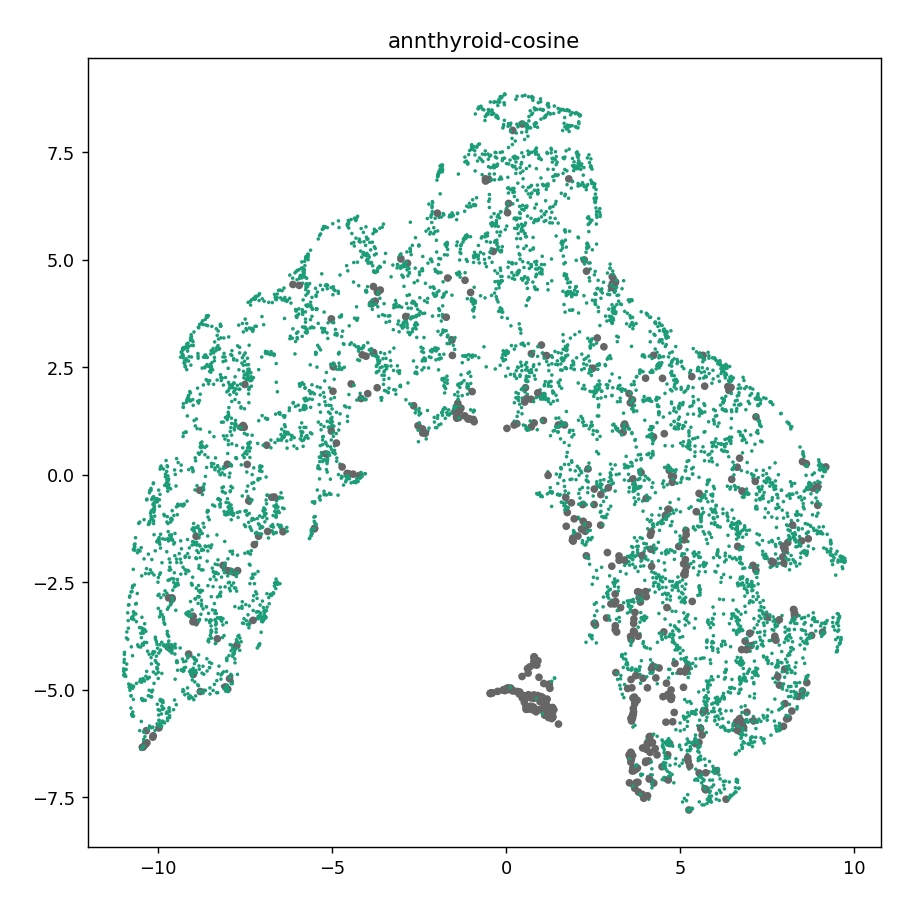
\includegraphics[width=2in]{images/umaps/annthyroid-cosine-umap2d.png}
%    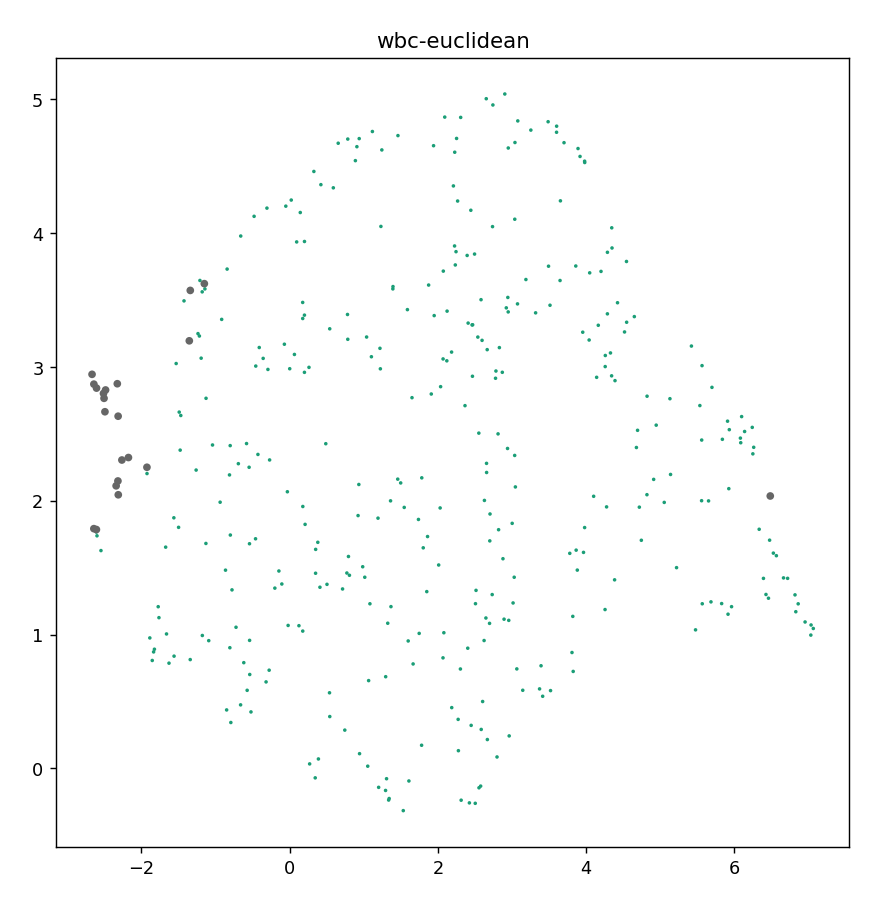
\includegraphics[width=2in]{images/umaps/wbc-euclidean-umap2d.png}
%    \caption{UMAP projection of Annthyroid (left) and WBC (right). Anomalies are in gray. Note that for Annthyroid, while there is a cluster of anomalies off the main manifold, many anomalies are distributed throughout the manifold. For WBC, the anomalies tend to be at the edge of the manifold.}
%    \label{fig:conclusions:umap-embeddings}
% \end{figure*}

\subsection{Future Directions}
\label{subsec:discussion:duture-directions}

The choice of distance function seems to have a significant impact on anomaly-detection performance.
In this case, domain knowledge is likely the best way to determine the distance function of choice.
Future work should explore a more diverse collection of domain-appropriate distance functions, such as Wasserstein distance on images, Levenshtein edit distance on strings, and Jaccard Index on the Maximal Common Sub-Graph of molecular structures.

Since CHAODA is highly effective on high-dimensional datasets, we can apply it to study Neural Networks.
We can create a dataset where each datum represents the activations of a neural network from an input to the neural network.
After mapping the manifold of such activations, we can detect malicious inputs to neural networks based on the intuition that malicious inputs produce atypical activation patterns.

\subsection{Conclusion}
\label{subsec:discussion:conlcusion}

In conclusion, we have demonstrated that by mapping the manifolds occupied by data, we can exploit that knowledge to implement simple algorithms capable of outperforming other state-of-the-art approaches to anomaly detection.

    \section{Acknowledgements}
\label{sec:acknowledgements}

TODO

% The authors would like to thank the members of CSC 592 - Algorithms for Big Data for helpful feedback and discussions.
% We have been Clearly Hoping that Our Work Detects Anomalies.


    % \afterpage{\clearpage}
    \bibliographystyle{IEEEtran}
    \bibliography{references}
\end{document}
